\documentclass[a4paper,15pt]{article}
\usepackage{amssymb}
\usepackage{amsmath}
\usepackage[english, polish]{babel}
\usepackage[utf8]{inputenc}   % lub utf8
\usepackage[T1]{fontenc}
\usepackage{graphicx}
\usepackage{anysize}
\usepackage{enumerate}
\usepackage{times}
\usepackage{caption}
\usepackage{titlesec}
\usepackage{float}
\usepackage{titleps,kantlipsum}
\usepackage{listings}
\usepackage{xcolor}
\usepackage{hyperref}
\usepackage{framed}
\usepackage{tcolorbox}
\lstloadlanguages{Matlab}
\usepackage{lstlinebgrd}
 
\usepackage[justification=centering]{caption}
\titlelabel{\thetitle.\quad}

\pagenumbering{arabic}

\DeclareCaptionFont{white}{\color{white}}
\DeclareCaptionFormat{listing}{%
  \parbox{\textwidth}{\colorbox{darkgreen}{\parbox{\textwidth}{#1#2#3}}\vskip-4pt}}
\captionsetup[lstlisting]{format=listing,labelfont=white,textfont=white}
\lstset{frame=lrb,xleftmargin=\fboxsep,xrightmargin=-\fboxsep}

% Definicja nowego stylu strony
\newpagestyle{mypage}
{
  \headrule
  
  \sethead
  { \MakeUppercase{\thesection\quad \sectiontitle} } 
  {}
  {\thesubsection\quad \subsectiontitle}
  
  \setfoot
  {}
  {}
  {\thepage}
}

\newpagestyle{mypage_1}
{
	\headrule
	
	\sethead
	{  }
	{\MakeUppercase{Systemy Operacyjne - Laboratorium}}
	{}
	
	\setfoot
	{}
	{\thepage}
	{}
}

\settitlemarks{section,subsection,subsubsection}

\pagestyle{mypage_1}

\newcommand{\ask}[2]{
    \begin{tcolorbox}[colback=black!5!white,colframe=gray,title={Pytanie #1}]
        #2
    \end{tcolorbox}
}

\newcommand{\assignment}[2]{
    \begin{tcolorbox}[colback=black!5!white,colframe=black,title={Zadanie #1}]
        #2
    \end{tcolorbox}
}

%\marginsize{left}{right}{top}{bottom}
\marginsize{3cm}{3cm}{3cm}{3cm}
\sloppy
\titleformat{\section}
  {\normalfont\Large\bfseries}{\thesection}{1em}{}[{\titlerule[0.8pt]}]
 
\definecolor{darkred}{rgb}{0.9,0,0}
\definecolor{grey}{rgb}{0.4,0.4,0.4}
\definecolor{orange}{rgb}{1,0.6,0.05}
\definecolor{darkgreen}{rgb}{0.2,0.5,0.05}
\definecolor{babyblueeyes}{rgb}{0.63, 0.79, 0.95}
\definecolor{gainsboro}{rgb}{0.86, 0.86, 0.86}
 
\definecolor{mGreen}{rgb}{0,0.6,0}
\definecolor{mGray}{rgb}{0.5,0.5,0.5}
\definecolor{mPurple}{rgb}{0.58,0,0.82}
\definecolor{mKeyword}{RGB}{0,0,242}
\definecolor{backgroundColour}{RGB}{242,242,242}
\definecolor{frenchlilac}{rgb}{0.53, 0.38, 0.56}

\lstdefinestyle{CStyle}{
    backgroundcolor=\color{backgroundColour},   
    commentstyle=\color{mGreen},
    keywordstyle=\color{mKeyword},
    numberstyle=\tiny\color{mGray},
    stringstyle=\color{mPurple},
    basicstyle=\footnotesize,
    breakatwhitespace=false,         
    breaklines=true,                 
    %captionpos=b,                    
    keepspaces=true,                 
    numbers=left,                    
    numbersep=5pt,                  
    showspaces=false,                
    showstringspaces=false,
    showtabs=false,                  
    tabsize=2,
    language=C
}


\newcommand{\Hilight}{\makebox[0pt][l]{\color{cyan}\rule[-4pt]{0.65\linewidth}{14pt}}}


\begin{document}

\begin{table}
\begin{center}
\begin{tabular}{|c|c|c|}
\hline
\multicolumn{3}{|c|}{\textbf{Zaawansowana komunikacja międzyprocesowa - łącza nazwane, kolejki komunikatów}} \\ \hline Dominik Wróbel & 09 V 2019 & Czw. 17:00 \\ \hline

\end{tabular}
\end{center}
\end{table}

\tableofcontents

\newpage
\section{Łącza nazwane w powłoce}


\assignment{ - Łącza nazwane w powłoce}{ 
...otwieramy dwie powłoki - tak aby procesy które będą się komunikowały nie miały wspólnego przodka w którym zostało utworzone łącze komunikacyjne i aby wykluczyć dziedziczenie deskryptorów plików. \\
W dowolnej z nich tworzymy kolejkę FIFO o nazwie test \\
mkfifo test \\
W pierwszej z nich uruchamiamy program ls z parametrami -la i przekierowujemy standardowe wyjście tego polecenia na utworzoną kolejkę: \\
ls -la > test \\
W drugiej z nich uruchamiamy program grep z filtrem d i przekierowujmy jego standardowe wejście na utworzoną kolejkę: \\
grep d < test
}


\begin{figure}[H]
\centerline{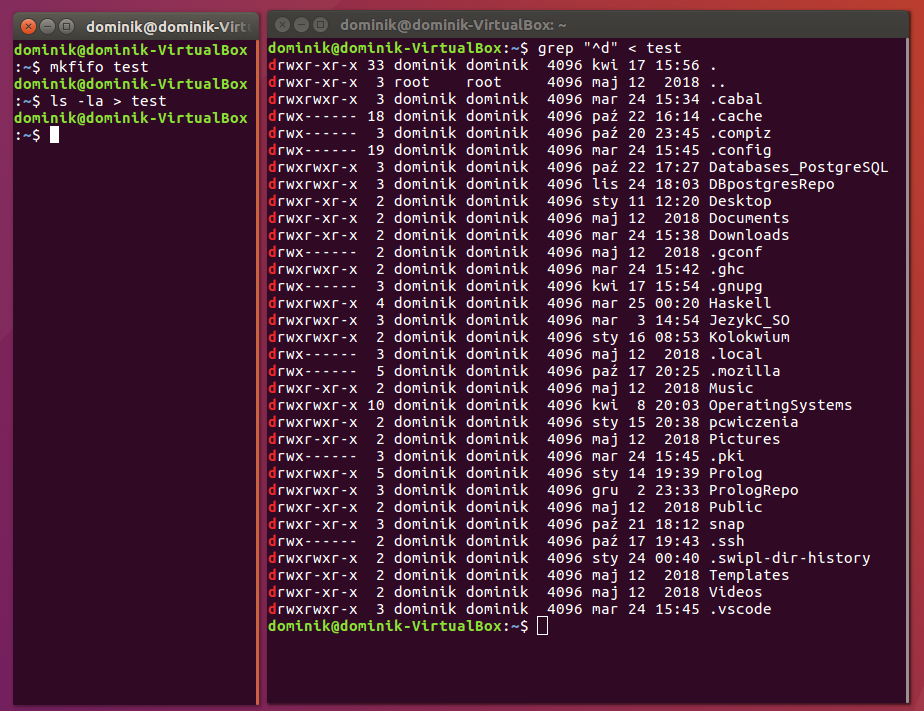
\includegraphics[scale=0.5]{zad1.png}}
\caption{FIFO w powłoce}
\label{fig:nazwane}
\end{figure}


\section{Łącza nazwane w API}

\subsection{Zadanie 1}

\assignment{1}{ 
W pierwszym programie proszę wprowadzić modyfikację tak aby:
\begin{itemize}
\item Serwer po uruchomieniu nie zatrzymywał się na otwieraniu łącza czytania danych od klienta, tylko przechodził do oczekiwania na dane od klienta.
\item Klient po wysłaniu komunikatu nie zatrzymywał się na otwieraniu łącza czytania danych od serwera, tylko przechodził do oczekiwania na dane od serwera.
\end{itemize}
}

W kodzie serwera i klienta dodano flagę O\_NONBLOCK przy otwieraniu pliku do czytania, aby nie zatrzymywać programu na otwieraniu deskryptora. Następnie flaga ta jest ponownie przywracana aby zatrzymać się na czytaniu danych. Otwierany jest również deskryptor pliku do zapisywania aby nie uzyskać EOF. Zmiany zaznaczono kolorem szarym w kodzie.


\begin{lstlisting}[style=CStyle, label=some-code, caption=srvfifo.c,
linebackgroundcolor={
	\ifnum\value{lstnumber}=3\color{gainsboro}\fi
	\ifnum\value{lstnumber}=13\color{gainsboro}\fi
	\ifnum\value{lstnumber}=14\color{gainsboro}\fi
	\ifnum\value{lstnumber}=15\color{gainsboro}\fi
	\ifnum\value{lstnumber}=18\color{gainsboro}\fi
	}
	]
	
  ... 
  fdsrv = open(fifosrvname, O_RDONLY | O_NONBLOCK); // setting nonblock flag 
  printf("After read opening\n");

  if(fdsrv == -1)
    {
      printf("FAIL!\nError: \'%s\'\n", strerror(errno));
      return 0;
    }
  printf("OK\n");

  flags = fcntl(fdsrv, F_GETFL); // reset nonblock flag
  flags &= ~O_NONBLOCK;
  fcntl(fdsrv, F_SETFL, flags);

  printf("Opening for writing");
  fdwrite = open(fifosrvname, O_WRONLY); // keep writing descriptor open

  while(1)
  {
  	...
	
\end{lstlisting}


\begin{lstlisting}[style=CStyle, label=some-code, caption=cntfifo.c,
linebackgroundcolor={
	\ifnum\value{lstnumber}=6\color{gainsboro}\fi
	\ifnum\value{lstnumber}=15\color{gainsboro}\fi
	\ifnum\value{lstnumber}=16\color{gainsboro}\fi
	\ifnum\value{lstnumber}=17\color{gainsboro}\fi
	\ifnum\value{lstnumber}=19\color{gainsboro}\fi
	}
	]

	...	

	printf("OK\nOpening client fifo queue \'%s\' for reading...", fifocntname);
      
    fdcnt = open(fifocntname, O_RDONLY | O_NONBLOCK);
      
    if(fdcnt == -1)
    {
      printf("FAIL!\nError: %s\n", strerror(errno));
      break;
    }

    // unblock 
    flags = fcntl(fdcnt, F_GETFL);
    flags &= ~O_NONBLOCK;
    fcntl(fdcnt, F_SETFL, flags);

    fdwrite = open(fifocntname, O_WRONLY);
    printf("OK\n");



    /* Reading responce */
    printf("Waiting for data...");
	bread = read(fdcnt, &msg, sizeof(msg));

...
\end{lstlisting}

\subsection{Zadanie 2}

\ask{- Zadanie 2.1}{ 
Program 3. zawiera błąd: \\
Na czym on polega?
}

Błąd znajduje się w dwóch miejscach każdego z programów  (klienta i serwera), w obu programach są to dwa te same błędy.
\begin{itemize}
\item Zarówno w kliencie jak i serwerze nie uwzględniono przy otwieraniu kolejki do czytania maksymalnego rozmiaru wiadomości, \underline{który musi być mniejszy od rozmiaru} wysyłanej wiadomości.
\item Przy zapisie wiadomości korzysta się z sizeof dla struktury, w tym przypadku zwraca to wartość ponad limit i skutkuje błędem 'message too long'
\end{itemize}


\ask{- Zadanie 2.2}{ 
Program 3. zawiera błąd: \\
Jak go naprawić?
}
\begin{itemize}
\item Pierwszy z błędów należy naprawić ustawiając parametry struktury mq\_attr na takie aby maksymalny rozmiar wiadomości był mniejszy od rozmiaru bufora. 
\item Drugi z błędem naprawiamy poprzez ograniczenia rozmiaru wysyłane wiadomości przy wysyłania
\end{itemize}

\begin{lstlisting}[style=CStyle, label=some-code, caption=Poprawiony kod POSIX,
linebackgroundcolor={
	\ifnum\value{lstnumber}=13\color{gainsboro}\fi
	\ifnum\value{lstnumber}=27\color{gainsboro}\fi
	\ifnum\value{lstnumber}=34\color{gainsboro}\fi
	\ifnum\value{lstnumber}=40\color{gainsboro}\fi
	}
	]
	
  ...
  // SERWER
  struct mq_attr attr;
  attr.mq_flags = 0;
  attr.mq_maxmsg = 10;
  attr.mq_msgsize = 99;
  attr.mq_curmsgs = 0;
  
  /* Opening server psx queue */
  printf("Opening server queue \'%s\' for reading...", srvpsxqname);
  mq_unlink(srvpsxqname);
  qdsrv = mq_open(srvpsxqname, O_RDONLY | O_CREAT, PERM_FILE, &attr);  
  ...
  
  ...
  // KLIENT
  struct mq_attr attr;
  attr.mq_flags = 0;
  attr.mq_maxmsg = 10;
  attr.mq_msgsize = 99;
  attr.mq_curmsgs = 0;

  /* Opening client queue for reading  */
  printf("Opening client queue \'%s\' for reading...", cntpsxqname);
  mq_unlink(cntpsxqname);
  qdcnt = mq_open(cntpsxqname, O_RDONLY | O_CREAT, PERM_FILE, &attr);
  if(qdcnt == -1)
  
  ...
  // SERWER
  /* Sending responce */
  printf("OK\nWritting responce to client %ld...", (long)msg.pid);
  bwrite = mq_send(qdcnt, (const char*)&msg, 99, 0);  
  
  
  ...
  // KLIENT
  printf("Writting message...");
  bwrite = mq_send(qdsrv, (const char*)&msg, 99, 0);
  if(bwrite == -1)  
  

\end{lstlisting}



\ask{- Zadanie 2.3}{ 
Gdzie można sprawdzić limity ilości i rozmiaru wiadomości?
}

Można to zrobić przy użyciu funkcji mq\_getattr, przekazując do niej strukturę mq\_attr oraz deskryptor kolejki wiadomości. 

\begin{lstlisting}[style=CStyle, label=some-code,
linebackgroundcolor={
	\ifnum\value{lstnumber}=13\color{gainsboro}\fi
	\ifnum\value{lstnumber}=27\color{gainsboro}\fi
	\ifnum\value{lstnumber}=34\color{gainsboro}\fi
	\ifnum\value{lstnumber}=40\color{gainsboro}\fi
	}
	]
	
mq_getattr-get message-queue attributes
#include <mqueue.h>
int mq_getattr( 
	mqd_t mqd, /* message-queue descriptor */ 
	struct mq_attr *attr /* attributes */ 
); /* Returns 0 on success or -1 on error (sets errno) */
\end{lstlisting}


\section{Chatbot Eliza}

W tym zadaniu zaimplementowano chatbot Eliza przy użyciu komunikacji opartej na kolejkach FIFO. Kod zamieszczono poniżej

\begin{lstlisting}[style=CStyle, label=some-code, caption=srveliza.c]

#include <stdlib.h>
#include <stdio.h>
#include <errno.h>
#include <fcntl.h>
#include <string.h>
#include <ctype.h>

#include <sys/types.h>
#include <sys/stat.h>
/* ------------------------------------------------------------- */

#include "fifo.h"
/* ------------------------------------------------------------- */

#define MAX 100
#define SHORT 10
#define VERYSHORT 2

char *response[]= {
     "How are you this beautiful day ?",
     "Did you have a happy childhood ?",
     "Did you hate your father ?",
     "Did you have a good friend ?",
     "Did you like your friend ?",
     "What do you think about your friendship ?",
     "I'm not sure I understand .",
     ""
};

char *trans[]={
     "no","Tell me more about the detail .",
     "yes","Tell me more about the detail .",
     "fuck","Don't be so rude again !",
     "shet","Don't be so rude again !",
     "you","Let't not talk about me .",
     "think","Why do you think that ?",
     "hate","So you hate something -- tell me more .",
     "what","Why do you ask ?",
     "want","Why do you want that ?",
     "need","We all need many things -- is this special ?",
     "why","Remember,therapy is good for you .",
     "know","How do you know that ?",
     "bye","Your bill will be mailed to you .",
     "murder","I don't like killing .",
     "kill","It is wrong to kill .",
     "jerk","Don't ever call me a jerk !",
     "can't","Don't be negative -- be positive .",
     "failure","Strive for success .",
     "never","Don't be negative -- be positive .",
     "unhappy","Why are you unhappy ?",
     "beautiful","I'm sure you like her,don't you ?",
     "like","Why do you like that?",
     "love","Remember,love everthing what you love .",
     ""
};

char topics[MAX][80];
char token[80];
char *p_pos;
int res=0;
int head=0;
int tail=0;

void assert_topic(char *);
void get_token(void);
int is_in(char, char *);
int lookup(char *);
int find_topic(char *);
int in_topics(char *);

/* creat the doctor's response */
char* respond (char *s)
{
    char t[80];
    char *ret;
    int loc;
    if (strlen(s)<VERYSHORT && strcmp(s,"bye"))  {
       if (find_topic(t))  {
          printf ("You just said:");
          printf ("%s\n",t);
          printf ("tell me more .\n");
       }
       else {
          if (!*response[res])  res=0;   /* start over again */
          /*printf ("%s\n",response[res++]);*/
	  ret = response[res++];
	  
       }
       return ret;
    }
    if (in_topics(s))  {
       /* printf ("Stop repeating yourself !\n"); */
      ret = "Stop repeating yourself !\n";
      return ret;
    }
    if (strlen(s)>SHORT) assert_topic(s);
    do {
       get_token();
       loc=lookup(token);
       if (loc!=-1)  {
	  /* printf ("%s\n",trans[loc+1]); */
	  ret = trans[loc+1];
          return ret;
       }
    } while (*token);
    /* comment of last resort */
    if (strlen(s)>SHORT)
       /* printf ("It's seem intersting , tell me more ...\n"); */
      ret = "It's seem intersting , tell me more ...\n";
    /* else printf ("Tell me more ...\n"); */
    else ret = "Tell me more ...\n";

return ret;
}

/* Lookup a keyword in translation table  */
int lookup (char *token)
{
    int t;
    t=0;
    while (*trans[t])  {
          if (!strcmp (trans[t],token))  return t ;
          t++;
    }
    return -1;
}

/* place a topic into the topics database  */
void assert_topic (char *t)
{
    if (head==MAX)  head=0;  /* wrap around */
    strcpy(topics[head],t);
    head++;
}

/* retrieve a topic  */
int find_topic (char *t)
{
    if (tail!=head)  {
       strcpy(t,topics[tail]);
       tail++;
       /* wrap around if necessary */
       if (tail==MAX) tail=0;
       return 1;
    }
    return 0;
}

/* see if in topics queue */
int in_topics (char *s)
{
    int t;
    for (t=0;t<MAX;t++)
        if (!strcmp(s,topics[t]))  return 1;
    return 0;
}

/* return a token from the input stream */
void get_token (void)
{
    char *p;
    p=token;
    /* skip spaces */
    while (*p_pos==' ') p_pos++;

    if (*p_pos=='\0') {  /*is end of input*/
       *p++='\0';
       return;
    }
    if (is_in(*p_pos,".!?")) {
       *p=*p_pos;
       p++,p_pos++;
       *p='\0';
       return ;
    }

    /*read word until*/
    while(*p_pos!=' '&&!is_in(*p_pos,".,;?!")&&*p_pos)  {
         *p=tolower(*p_pos++);
         p++;
    }
    *p='\0';
}

int is_in(char c, char *s)
{
    while(*s) {
       if(c==*s) return 1;
       s++;
    }
    return 0;
}



int main(void)
{
  struct message msg;
  char* fifosrvbasename = "srvfifoqueue";
  char fifosrvname[FIFO_NAME_BUF_SIZE];
  char fifocntname[FIFO_NAME_BUF_SIZE];
  int fdsrv,
    fdcnt,
    bread,
    bwrite,
    fdsrv_w;
  
  printf("Server started...\n");
  setbuf(stdout, NULL);

  /* Creating server fifo queue */
  make_srv_fifo_queue_name(fifosrvname, fifosrvbasename, FIFO_NAME_BUF_SIZE);
  printf("Creating server fifo queue \'%s\'...", fifosrvname);
  if((mkfifo(fifosrvname, PERM_FILE) == -1) && (errno != EEXIST))
    {
      printf("FAIL!\nError: %s\n", strerror(errno));
      return 0;
    }

  /* Opening fifo */
  printf("OK\nOpening server fifo queue \'%s\' for reading...", fifosrvname);
  /* O_NONBLOCK - added */
  fdsrv = open(fifosrvname, O_RDONLY|O_NONBLOCK);
  if(fdsrv == -1)
    {
      printf("FAIL!\nError: \'%s\'\n", strerror(errno));
      return 0;
    }


  int flags= fcntl(fdsrv,F_GETFL);
  flags &= ~O_NONBLOCK;
  fcntl(fdsrv,F_SETFL,flags);
  //otworzenie do zapisu
  fdsrv_w = open(fifosrvname, O_WRONLY);
  if(fdsrv_w == -1)
    {
      printf("FAIL!\nError: \'%s\'\n", strerror(errno));
      return 0;
    }

  printf("OK\n");

  while(1)
    {
      /* Reading from queue */
      printf("Waiting for data...");
      bread = read(fdsrv, &msg, sizeof(msg));
      if(bread == -1)
	{
	  printf("FAIL!\nError: %s\n", strerror(errno));
	  break;
	}
      printf("OK\n");

      printf("Message from client [%d]: %s\n", msg.pid, msg.data);
     
      /* printf("Your responce: ");
      stdin_readall(msg.data, MESSAGE_BUF_SIZE);
      */

      /* Creating client fifo name  */
      make_cnt_fifo_queue_name(fifocntname, msg.pid, FIFO_NAME_BUF_SIZE); 

      /* Opening client fifo for writing  */
      printf("Opening client fifo \'%s\' for writing...", fifocntname);
      fdcnt = open(fifocntname, O_WRONLY);
      if(fdcnt == -1)
	{
	  printf("FAIL!\nError: %s\n", strerror(errno));
	  break;
	}




      /*Sending responce*/
      p_pos = msg.data;
      /* printf("odpowiedz: %s", respond(msg.data)); */
      strcpy(msg.data, respond(msg.data));
      printf("OK\nWritting responce to client [%ld]...", (long)msg.pid);
      bwrite = write(fdcnt, &msg, sizeof(msg));
      if(bwrite == -1)
	{
	  printf("FAIL!\nError: %s\n", strerror(errno));
	  break;
	}
      printf("OK\n");
      close(fdcnt);
    }
  
  
  /* Cleaning up */
  close(fdsrv);
  unlink(fifosrvname);
  
  return 0;
}



\end{lstlisting}

\begin{lstlisting}[style=CStyle, label=some-code, caption=cnteliza.c]
	

#include <stdlib.h>
#include <stdio.h>
#include <errno.h>
#include <fcntl.h>

#include <sys/types.h>
#include <sys/stat.h>

#include "fifo.h"
/* ------------------------------------------------------------- */

int main(void)
{
  struct message msg;
  char* fifosrvbasename = "srvfifoqueue";
  char fifosrvname[FIFO_NAME_BUF_SIZE];
  char fifocntname[FIFO_NAME_BUF_SIZE];
  int fdsrv,
    fdcnt,
    bread,
    bwrite,
    fdcnt_w;
  
  printf("Client [%ld] started...\n", (long)getpid());
  setbuf(stdout, NULL);
  msg.pid = getpid();

  /* Creating client fifo name */
  make_cnt_fifo_queue_name(fifocntname, msg.pid, FIFO_NAME_BUF_SIZE);
  printf("Creating client fifo queue \'%s\'...", fifocntname);
  if((mkfifo(fifocntname, PERM_FILE) == -1) && (errno != EEXIST))
    {
      printf("FAIL!\nError: %s\n", strerror(errno));
      return 0;
    }

  /* Opening server fifo for writing */
  make_srv_fifo_queue_name(fifosrvname, fifosrvbasename, FIFO_NAME_BUF_SIZE);
  printf("OK\nOpening server fifo queue \'%s\' for writing...", fifosrvname);
  fdsrv = open(fifosrvname, O_WRONLY);
  if(fdsrv == -1)
    {
      printf("FAIL!\nError: %s\n", strerror(errno));
      return 0;
    }
  printf("OK\n");

  while(1)
    {
      /* Getting message */
      printf("Send message: ");
      if(stdin_readall(msg.data, MESSAGE_BUF_SIZE) == 0)
	break;

      /* Sending message to server */
      printf("Writing message to server...");
      bwrite = write(fdsrv, &msg, sizeof(msg));
      if(bwrite == -1)
	{
	  printf("FAIL!\nError: %s\n", strerror(errno));
	  break;
	}

      /* Opening client fifo for reading */
      printf("OK\nOpening client fifo queue \'%s\' for reading...", fifocntname);
      fdcnt = open(fifocntname, O_RDONLY|O_NONBLOCK);
      if(fdcnt == -1)
	{
	  printf("FAIL!\nError: %s\n", strerror(errno));
	  break;
	}

	int flags= fcntl(fdcnt,F_GETFL);
	flags &= ~O_NONBLOCK;
	fcntl(fdcnt,F_SETFL,flags);
	//otworzenie do zapisu
	fdcnt_w = open(fifocntname, O_WRONLY);
	if(fdcnt_w == -1)
	{
	printf("FAIL!\nError: \'%s\'\n", strerror(errno));
	return 0;
	}

      printf("OK\n");
      
      /* Reading responce */
      printf("Waiting for data...");
      bread = read(fdcnt, &msg, sizeof(msg));
      if(bread == -1)
	{
	  printf("FAIL!\nError: %s\n", strerror(errno));
	  close(fdcnt);
	  break;
	}
      close(fdcnt);
      printf("OK\nMessage from server: %s\n", msg.data);
    }

  /* Cleaning up */
  close(fdsrv);
  unlink(fifocntname);

  return 0;
}



\end{lstlisting}


\end{document}
